% Бүлэг 1

\chapter{Платформ хөгжүүлэх онол, арга зүйн судалгаа}
\label{Chapter1}

\section{Бүлгийн зорилго ба судалгааны хүрээ}
Энэ бүлэг нь Anoce буюу Монголын загварын архивын веб платформыг хөгжүүлэх үндэслэл, төслийн үүсэл, хэрэглэгчийн хэрэгцээ, шаардлага болон сонгосон хөгжүүлэх арга зүйг тайлбарлана. Системийн техникийн хэрэгжилт дараагийн бүлгүүдэд дэлгэрэнгүй орох тул энэ бүлэгт \textit{“яагаад ийм архивын платформ хэрэгтэй вэ, ямар ижил төстэй системүүдтэй харьцуулж болох вэ, ямар арга зүйгээр хөгжүүлэх нь зохистой вэ?”} гэсэн асуултад хариулна.

Судалгааны хүрээг дараах байдлаар тогтоов.
\begin{itemize}
  \item Монголын загварын мэдээллийг дижитал архив болгон бүтэцжүүлэх хэрэгцээг тодорхойлох;
  \item Public archive, editorial site, headless CMS, global search, AI assistant бүхий системүүдийн нийтлэг шинжийг судлах;
  \item Зочин, бүртгэлтэй хэрэглэгч, редактор, админ, систем хөгжүүлэгчийн хэрэгцээг шинжлэх;
  \item Функциональ болон функциональ бус шаардлагын эхний түвшний жагсаалт гаргах;
  \item Agile, Prototype, Spiral, Kanban, Design Science Research зэрэг аргачлалыг харьцуулж, төслийн нөхцөлд тохирох хосолсон арга зүй сонгох.
\end{itemize}

\section{Төслийн үүсэл, хөгжлийн түүх}
Төсөл нь анх Монголын загварын брэнд, collection, editorial content-ийг визуал төвтэй байдлаар харуулах вебсайт гэсэн санаанаас эхэлсэн. Хөгжүүлэлтийн явцад зөвхөн static showcase бус, харин content repository, admin CMS, global search, Supabase authentication, bookmark/follow, RAG chatbot, asset management бүхий илүү бүрэн платформ болж өргөжив. Репозиторийн route, library, seed script, diagram бүтэц нь энэ төслийг нэг мэдээллийн системийн артефакт гэж авч үзэх үндэслэл болно.

\begin{figure}[htbp]
  \centering
  \resizebox{\textwidth}{!}{\begin{tikzpicture}[x=1cm,y=1cm,>=latex]
  \tikzstyle{phase}=[draw, rounded corners=2pt, fill=blue!8, minimum width=3.2cm, minimum height=1.1cm, align=center]
  \tikzstyle{arrow}=[->, thick]

  \node[phase] (p1) at (0,0) {1-р үе шат\\Archive UX эхлэл};
  \node[phase] (p2) at (4.2,0) {2-р үе шат\\Domain model};
  \node[phase] (p3) at (8.4,0) {3-р үе шат\\CouchDB CMS};
  \node[phase] (p4) at (12.6,0) {4-р үе шат\\Search + AI};

  \draw[arrow] (p1) -- (p2);
  \draw[arrow] (p2) -- (p3);
  \draw[arrow] (p3) -- (p4);

  \node[align=center] at (0,-1.2) {Hero\\Collections grid};
  \node[align=center] at (4.2,-1.2) {Designer\\Collection\\Article};
  \node[align=center] at (8.4,-1.2) {Repository\\Admin CRUD};
  \node[align=center] at (12.6,-1.2) {Search overlay\\RAG chatbot};
\end{tikzpicture}
}
  \caption[Төслийн хөгжлийн үе шат]{Anoce/MFA платформын хөгжлийн үндсэн үе шат}
  \label{fig:project-timeline}
\end{figure}

\begin{longtable}{|L{0.12\textwidth}|L{0.22\textwidth}|L{0.27\textwidth}|L{0.25\textwidth}|}
  \caption{Төслийн хөгжлийн үе шат ба судалгааны утга}
  \label{tab:project-history}\\
  \hline
  \textbf{Үе шат} & \textbf{Гол зорилго} & \textbf{Бодит материал} & \textbf{Судалгааны ач холбогдол} \\ \hline
  I үе шат & Нүүр хуудас ба archive identity бүрдүүлэх & Hero, Discover, Collections grid, navigation & Визуал төвтэй fashion archive-ийн хэрэглэгчийн анхны сэтгэгдэл тодорсон. \\ \hline
  II үе шат & Domain content model үүсгэх & Designer, Collection, Look, Article, User type & Загварын өгөгдлийг нэг хэлбэрт оруулж, дахин ашиглах боломж бүрдсэн. \\ \hline
  III үе шат & Content repository ба public API холбох & CouchDB repository, \path{/api/content/*} routes & Static data-аас CMS-driven платформ руу шилжих суурь тавигдсан. \\ \hline
  IV үе шат & Admin CMS ба asset workflow хөгжүүлэх & Content CRUD, asset upload & Редакцийн ажлыг frontend кодоос салгаж, админ хэрэглэгч удирдах боломжтой болсон. \\ \hline
  V үе шат & Search ба AI туслах нэгтгэх & Search overlay, RAG seed, \path{/api/chat} & Archive discovery болон context-aware лавлах боломж нэмэгдсэн. \\ \hline
\end{longtable}

\section{Судалгааны асуудал}
Загварын архив нь энгийн article list-ээс ялгаатай. Нэг designer олон collection гаргана, collection бүр олон look-тэй, look бүр материал ба tag-тэй, нийтлэл нь дизайнер, collection, trend, зурагтай холбогдоно. Ийм өгөгдөл public user-д ойлгомжтой харагдах, редакторт засварлахад хялбар байх, API-аар тогтвортой дамжих, хайлт болон AI туслахад context болж ашиглагдах ёстой.

Энэхүү асуудлыг дараах түвшинд авч үзэв.
\begin{enumerate}
  \item \textbf{Архивын бүтэц:} дизайнер, collection, look, нийтлэл, asset хоорондын холбоог уян хатан боловч тогтвортой model-д оруулах шаардлагатай.
  \item \textbf{Редакцийн workflow:} article, designer, collection нэмэх, засах, review хийх, publish хийх ажиллагаа protected admin орчинд төвлөрөх ёстой.
  \item \textbf{Хэрэглэгчийн нээлт:} хэрэглэгч улирал, designer, материал, trend, article-аар хайж, шүүж, холбоотой content руу шилжих боломжтой байх шаардлагатай.
  \item \textbf{AI туслахын найдвартай байдал:} chatbot нь archive-д байхгүй мэдээллийг зохиохгүй, live content болон curated RAG context-д тулгуурлах ёстой.
\end{enumerate}

Иймээс судалгааны асуудлыг дараах байдлаар тодорхойлов.

\begin{quote}
Монголын загварын designer, collection, look, article, asset өгөгдлийг нэгтгэн хадгалах, удирдах, хайх, AI туслахаар лавлах боломжтой веб архивын платформыг хэрхэн хэрэглэгч төвтэй, өргөтгөх боломжтой, өгөгдлийн хяналттай байдлаар зохион бүтээх вэ?
\end{quote}

\section{Хэрэглэгч ба оролцогч талуудын шинжилгээ}
Систем нь public хэрэглэгчдэд архив үзэх, бүртгэлтэй хэрэглэгчдэд bookmark ба follow ашиглах, редактор ба админд content удирдах, хөгжүүлэгчид системийг өргөтгөх боломж олгоно.

\begin{table}[htbp]
  \centering
  \caption{Оролцогч талууд ба хэрэгцээ}
  \label{tab:stakeholders}
  \small
  \begin{tabular}{|L{0.17\textwidth}|L{0.33\textwidth}|L{0.36\textwidth}|}
    \hline
    \textbf{Оролцогч} & \textbf{Гол хэрэгцээ} & \textbf{Системийн хариу шийдэл} \\ \hline
    Зочин хэрэглэгч & Монголын дизайнер, collection, article, trend-тэй танилцах & Home, archive, designers, editorial, global search \\ \hline
    Бүртгэлтэй хэрэглэгч & Сонирхсон article/look хадгалах, брэнд дагах, профайл ашиглах & Supabase Auth, bookmark, follow, profile page \\ \hline
    Редактор & Нийтлэл бичих, зураг сонгох, publish status удирдах & Admin articles, review/edit page, asset library \\ \hline
    Админ & Designer, collection, user role, asset, content state удирдах & Protected admin dashboard, CRUD routes, role gate \\ \hline
    Систем хөгжүүлэгч & Модульчлагдсан, засварлахад ойлгомжтой codebase & Next.js App Router, repository abstraction, shared types \\ \hline
  \end{tabular}
\end{table}

\section{Функциональ шаардлагын эхний шинжилгээ}
Функциональ шаардлагыг тодорхойлохдоо хэрэглэгчийн үндсэн аялал, админ редакцийн ажил, өгөгдлийн загвар, хайлт болон AI туслахын хэрэглээг хамтад нь авч үзэв. Энэхүү систем нь зөвхөн мэдээлэл харуулах нүүр хуудас биш тул шаардлага бүрийг ``хэн ашиглах вэ'', ``ямар өгөгдөлд хүрэх вэ'', ``амжилттай ажилласныг яаж таних вэ'' гэсэн гурван өнцгөөс тодорхойлсон.

Шаардлагыг эхний түвшинд дараах бүлэгт ангилав.
\begin{itemize}
  \item Public archive шаардлага нь зочин хэрэглэгч дизайнер, коллекц, нийтлэл, look мэдээлэл үзэх болон хайх боломжийг хамарна.
  \item Редакцийн шаардлага нь админ болон редактор хэрэглэгч контент үүсгэх, засах, нийтлэх, asset удирдах урсгалыг хамарна.
  \item Хэрэглэгчийн хувийн шаардлага нь bookmark, follow, profile зэрэг бүртгэлтэй хэрэглэгчийн үйлдлийг хамарна.
  \item AI туслахын шаардлага нь архивын live content болон curated RAG dataset-д тулгуурлан асуултад хариулах үйл ажиллагааг хамарна.
  \item Өгөгдлийн pipeline шаардлага нь demo content, CouchDB seed, RAG import, search index шинэчлэлтийг хамарна.
\end{itemize}

\begin{longtable}{|L{0.08\textwidth}|L{0.25\textwidth}|L{0.12\textwidth}|L{0.41\textwidth}|}
  \caption{Системийн үндсэн функциональ шаардлага}
  \label{tab:functional-requirements}\\
  \hline
  \textbf{Код} & \textbf{Шаардлага} & \textbf{Priority} & \textbf{Тайлбар ба шалгах нөхцөл} \\ \hline
  FR-01 & Дизайнерын лавлах үзүүлэх & P1 & Designer profile, tier, bio, cover/profile image, social link мэдээлэл харагдана. Хэрэглэгч дизайнерын detail хуудас руу шилжиж чадна. \\ \hline
  FR-02 & Collection archive үзүүлэх & P1 & Collection-ийг designer, season, year, category, material-аар шүүх, detail хуудас нээх, related designer руу шилжих боломжтой байна. \\ \hline
  FR-03 & Look мэдээлэл хадгалах & P1 & Collection дотор look number, image, description, materials, tags хадгалж, UI дээр зураг болон metadata зэрэгцэн харагдана. \\ \hline
  FR-04 & Editorial article удирдах & P1 & Нийтлэл title, subtitle, category, body, cover image, status, tags, credits-тэй байна. Draft, review, published төлөвөөр ялгах боломжтой байна. \\ \hline
  FR-05 & Global search ажиллуулах & P1 & Article, collection, designer, brand өгөгдлийг нэг overlay дээр оноогоор эрэмбэлж харуулна. Query бичихэд debounce хийж, result бүлгээр ангилагдана. \\ \hline
  FR-06 & Хэрэглэгчийн bookmark/follow & P2 & Бүртгэлтэй хэрэглэгч article, look, brand хадгалж, profile хэсгээс дахин үзэх боломжтой байна. Зочин хэрэглэгч login шаардлагатайг ойлгомжтой харна. \\ \hline
  FR-07 & Admin CMS хамгаалах & P1 & Viewer бус role-той хэрэглэгчид article, collection, designer, asset, user удирдах боломжтой байна. API түвшинд 401/403 response зөв буцна. \\ \hline
  FR-08 & Asset upload ба serve хийх & P2 & CouchDB attachment эсвэл API-аар зурагт asset хадгалах, public URL хэлбэрээр article/collection/designer-д ашиглах боломжтой байна. \\ \hline
  FR-09 & AI chatbot асуултад хариулах & P2 & Live archive context болон RAG document ашиглан fashion archive-ийн асуултад хариулна. Context хүрэлцэхгүй үед зохиомол хариулт өгөхгүй. \\ \hline
  FR-10 & Seed/import pipeline & P2 & Demo content, CouchDB content, Supabase RAG document import хийх script-үүдтэй байна. Local demo орчин хурдан сэргээгдэх боломжтой байна. \\ \hline
\end{longtable}

\section{Функциональ бус шаардлагын эхний шинжилгээ}
Функциональ бус шаардлага нь системийн ``юу хийх вэ'' гэхээс илүү ``ямар чанартай ажиллах вэ'' гэсэн асуудлыг тодорхойлно. Anoce/MFA платформын хувьд визуал контент олон, admin үйлдэл protected, AI provider external, өгөгдөл хоёр backend-д хуваагдах тул usability, security, maintainability, data integrity, performance, AI reliability зэрэг чанарын шинжүүдийг эхний шатнаас тодорхойлох шаардлагатай.

Эдгээр шаардлагыг хэрэгжилтийн үед дараах байдлаар шалгана: public route нээгдэх хугацаа, mobile responsive харагдац, admin role gate, API response consistency, repository conversion logic, chatbot fallback, environment secret тусгаарлалт, table/diagram/documentation consistency. Нэг бүрийг production SLA түвшинд хэмжихээс илүү дипломын MVP-д тохирох бодит шалгуур болгон тодорхойлов.

\begin{table}[htbp]
  \centering
  \caption{Функциональ бус шаардлагын ангилал}
  \label{tab:nonfunctional-requirements}
  \begin{tabular}{|L{0.20\textwidth}|L{0.30\textwidth}|L{0.36\textwidth}|}
    \hline
    \textbf{Чанарын шинж} & \textbf{Шаардлагын утга} & \textbf{Төслийн хүрээнд хэрэгжүүлэх чиглэл} \\ \hline
    Ашиглахад хялбар байдал & Public archive, search overlay, admin form ойлгомжтой байх & Visual card, filter bar, empty/loading state, responsive layout, form label/error state \\ \hline
    Өгөгдлийн бүрэн байдал & Collection, look, article relation алдагдахгүй байх & Repository normalization, stable slug, required field validation, update үед \texttt{\_rev} хадгалах \\ \hline
    Аюулгүй байдал & Admin content зөвшөөрөлгүй өөрчлөгдөхгүй байх & Supabase Auth, profile role, protected admin route/API, provider key-г server-side байлгах \\ \hline
    Өргөтгөх чадвар & Шинэ content type, AI provider, search logic нэмэхэд хялбар байх & Repository abstraction, shared type, provider fallback, seed/import script тусгаарлах \\ \hline
    Гүйцэтгэл & Archive/search хуудас боломжийн хурдтай ажиллах & Search debounce, indexed CouchDB query, image asset reuse, client/server boundary тодорхойлох \\ \hline
    Итгэлцэл & AI хариулт архивт байхгүй баримт зохиохгүй байх & RAG context, live archive result, insufficient context message, fallback summary \\ \hline
    Засварлахад хялбар байдал & Код болон тайлангийн бүтэц ойлгомжтой байх & Route, component, repository, AI, seed pipeline-ийг тусдаа module болгон зохион байгуулах \\ \hline
    Хүртээмж ба responsive чанар & Mobile болон desktop хэрэглээнд текст, зураг, товч давхцахгүй байх & Responsive grid, readable font size, table/diagram resize, contrast шалгах \\ \hline
  \end{tabular}
\end{table}

\section{Ижил төстэй системүүдийн судалгаа}
Ижил төстэй системийг зөвхөн нэг төрлийн fashion website гэж авч үзвэл Anoce/MFA-ийн онцлог бүрэн харагдахгүй. Тиймээс Монголын загварын сайт, олон улсын runway/archive платформ, музейн дижитал коллекц, digital showcase, fashion search engine гэсэн бүлгээр шинжиллээ. Судалгааны гол зорилго нь яг ижил бүтээгдэхүүн олох бус, харин archive structure, visual presentation, navigation, metadata, search, content workflow-ийн сайн жишээг ялган авах юм.

\subsection{Монголын ижил төстэй вебүүд}
Монголын зах зээлд бүрэн хэмжээний ``Монголын загварын нэгдсэн дижитал архив'' хэлбэрийн сайт ховор боловч загварын брэнд, дизайнерын portfolio, concept store, e-commerce чиглэлийн сайтууд Anoce/MFA-д хэрэгтэй олон санаа өгч байна. Amulet Mongolia нь дизайнерын уран сайхны portfolio болон collection story-г харуулдаг \cite{amulet_mongolia_site}. Deel by Michel \& Amazonka нь үндэсний хувцас, гар урлал, heritage narrative-ийг modern brand presentation-тай холбодог \cite{deel_brand_site}. Gobi Cashmere нь collection, category, product navigation-ийг тодорхой ангиллаар зохион байгуулсан e-commerce жишээ \cite{gobi_cashmere_site}. MongolianMade нь Монголд үйлдвэрлэсэн бүтээгдэхүүн, designer/artisan story-г concept store хэлбэрээр нэгтгэдэг \cite{mongolianmade_site}. Mongolian Gallery нь дизайнер брэнд, product filter, availability, brand filter зэрэг commerce metadata-г хэрэглэдэг \cite{mongolian_gallery_site}.

{\small
\begin{longtable}{|L{0.17\textwidth}|L{0.18\textwidth}|L{0.31\textwidth}|L{0.20\textwidth}|}
  \caption{Монголын ижил төстэй вебүүдийн шинжилгээ}
  \label{tab:mongolian-similar-systems}\\
  \hline
  \textbf{Вебсайт} & \textbf{Төрөл} & \textbf{Ажиллах зарчим ба UI шинж} & \textbf{Anoce/MFA-д авах санаа} \\ \hline
  Amulet Mongolia & Designer portfolio & Том зураг, collection story, gallery, minimal navigation ашиглаж дизайнерын identity-г онцолдог. UI нь artist portfolio мэдрэмжтэй, текст бага, зураг давамгай. & Designer profile болон collection story хэсэгт visual-first layout хэрэглэх. \\ \hline
  Deel by Michel \& Amazonka & Heritage fashion brand & Үндэсний хувцасны философи, flagship store, category navigation, appointment/contact урсгалтай. UI нь luxury brand-ийн цэвэр, editorial өнгөтэй. & Монгол соёлын тайлбарыг collection metadata болон editorial content-тэй холбох. \\ \hline
  Gobi Cashmere & Fashion e-commerce & Category, gender, season, product grid, sale navigation-оор хэрэглэгчийг бараа руу чиглүүлдэг. & Season/material filter-ийг ойлгомжтой харагдуулах. \\ \hline
  Mongolian Made & Concept store & Монгол брэндүүдийг ангилал, story, store location, gallery хэлбэрээр нэгтгэдэг. & Брэндийн гарал, designer story-г архивын тайлбарт тусгах. \\ \hline
  Mongolian Gallery & Designer brand shop & Product filter, brand filter, availability, sort, price зэрэг commerce metadata ашигладаг. UI нь grid, filter sidebar, product card дээр төвлөрдөг. & Archive grid-д filter/sort, entity metadata, card scanning pattern ашиглах. \\ \hline
\end{longtable}
}

\begin{figure}[htbp]
  \centering
  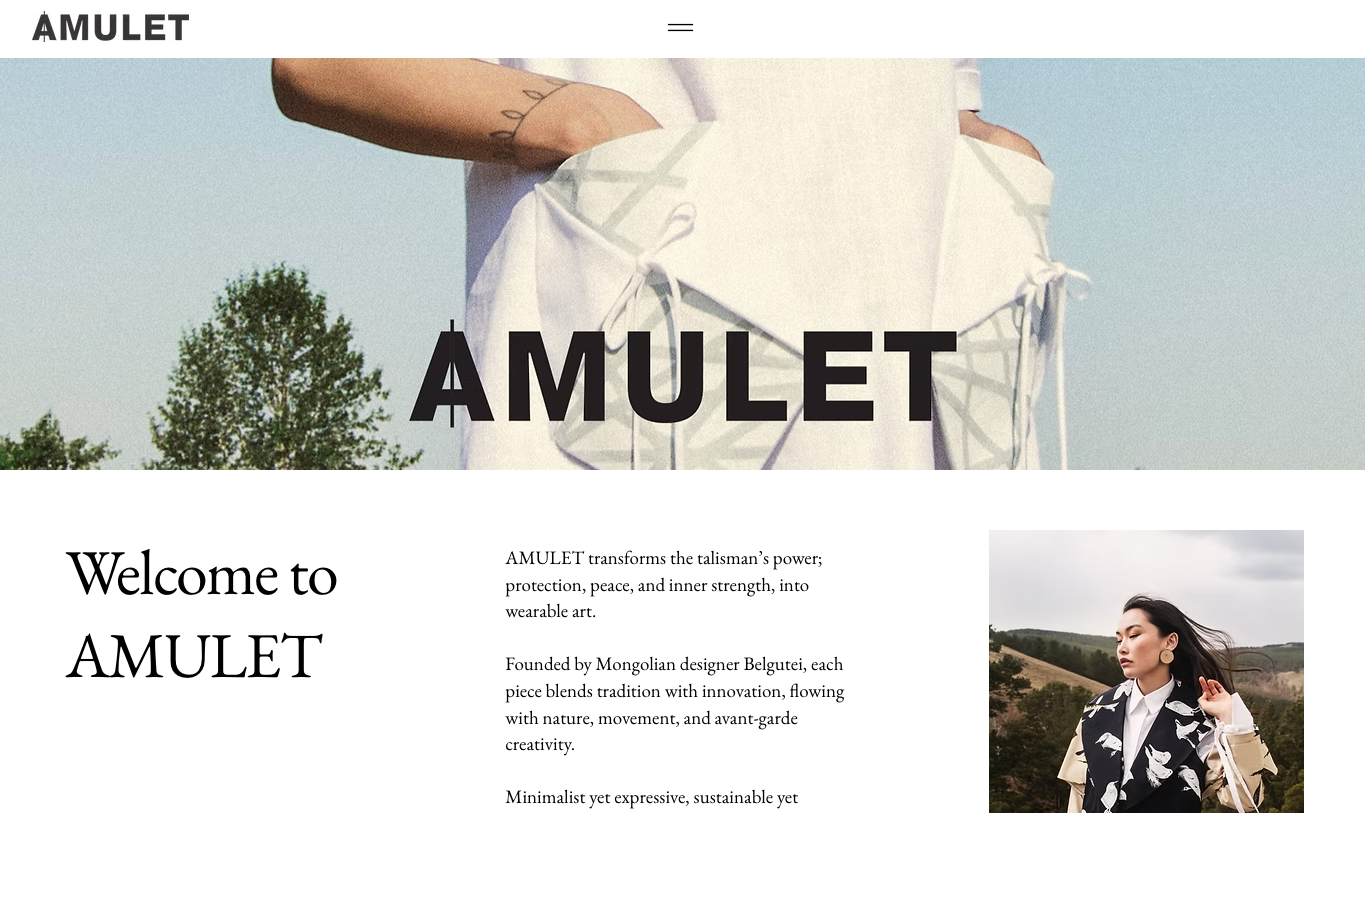
\includegraphics[width=0.31\textwidth]{Figures/similar_systems/amulet_mongolia.png}\hfill
  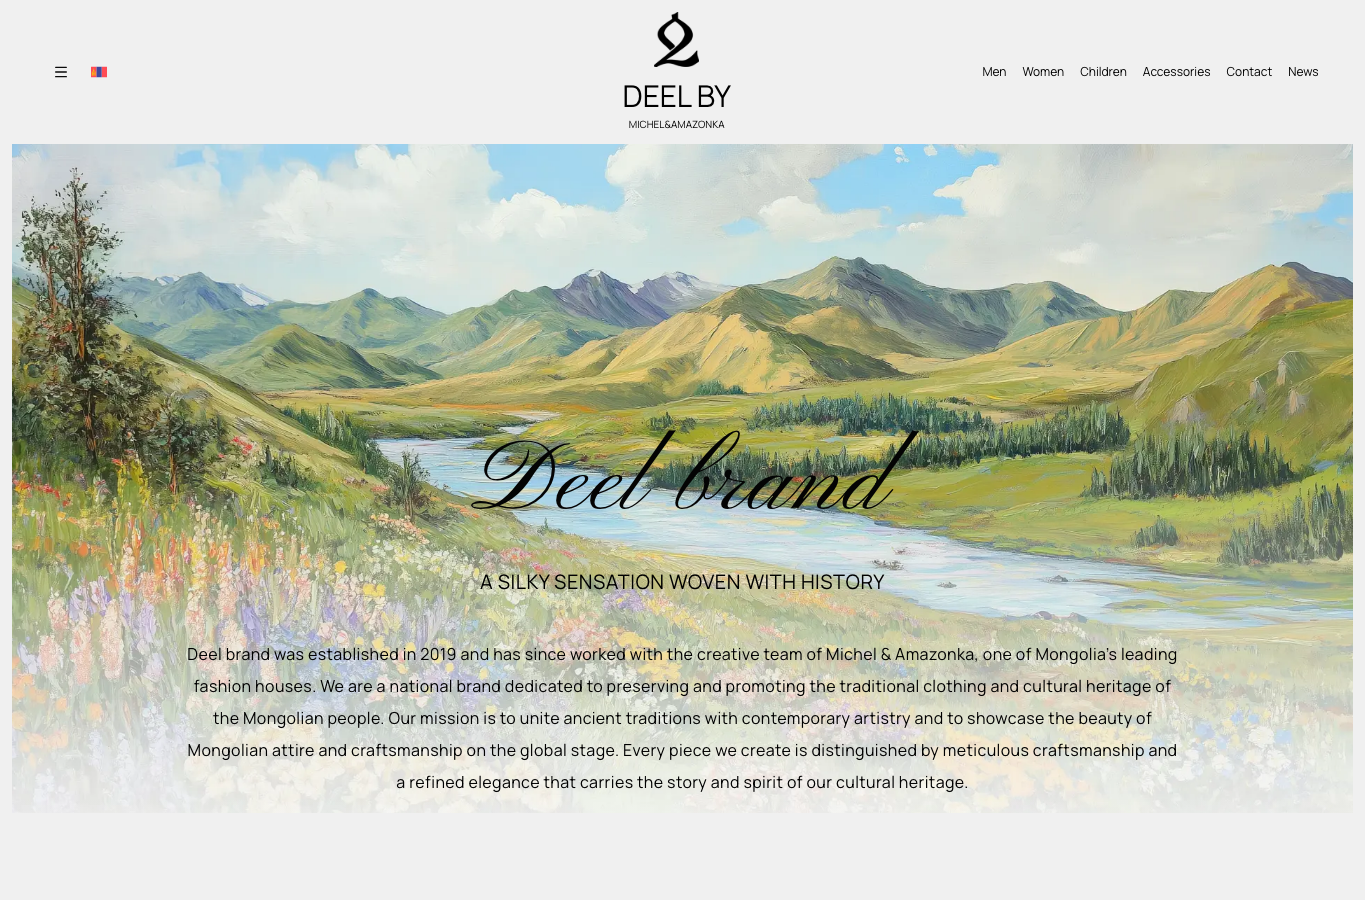
\includegraphics[width=0.31\textwidth]{Figures/similar_systems/deel_brand.png}\hfill
  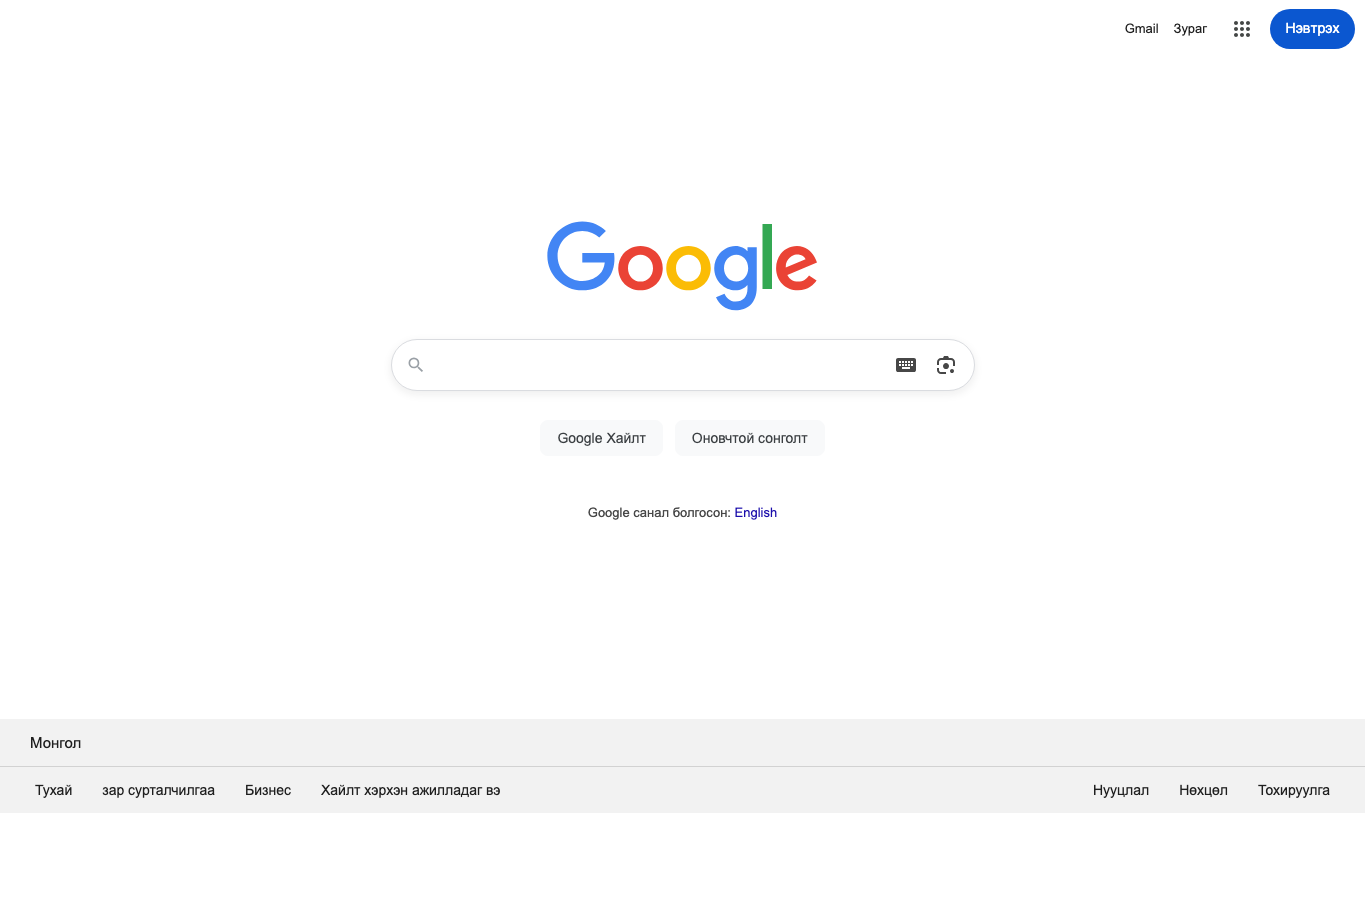
\includegraphics[width=0.31\textwidth]{Figures/similar_systems/gobi_cashmere.png}\\[0.6em]
  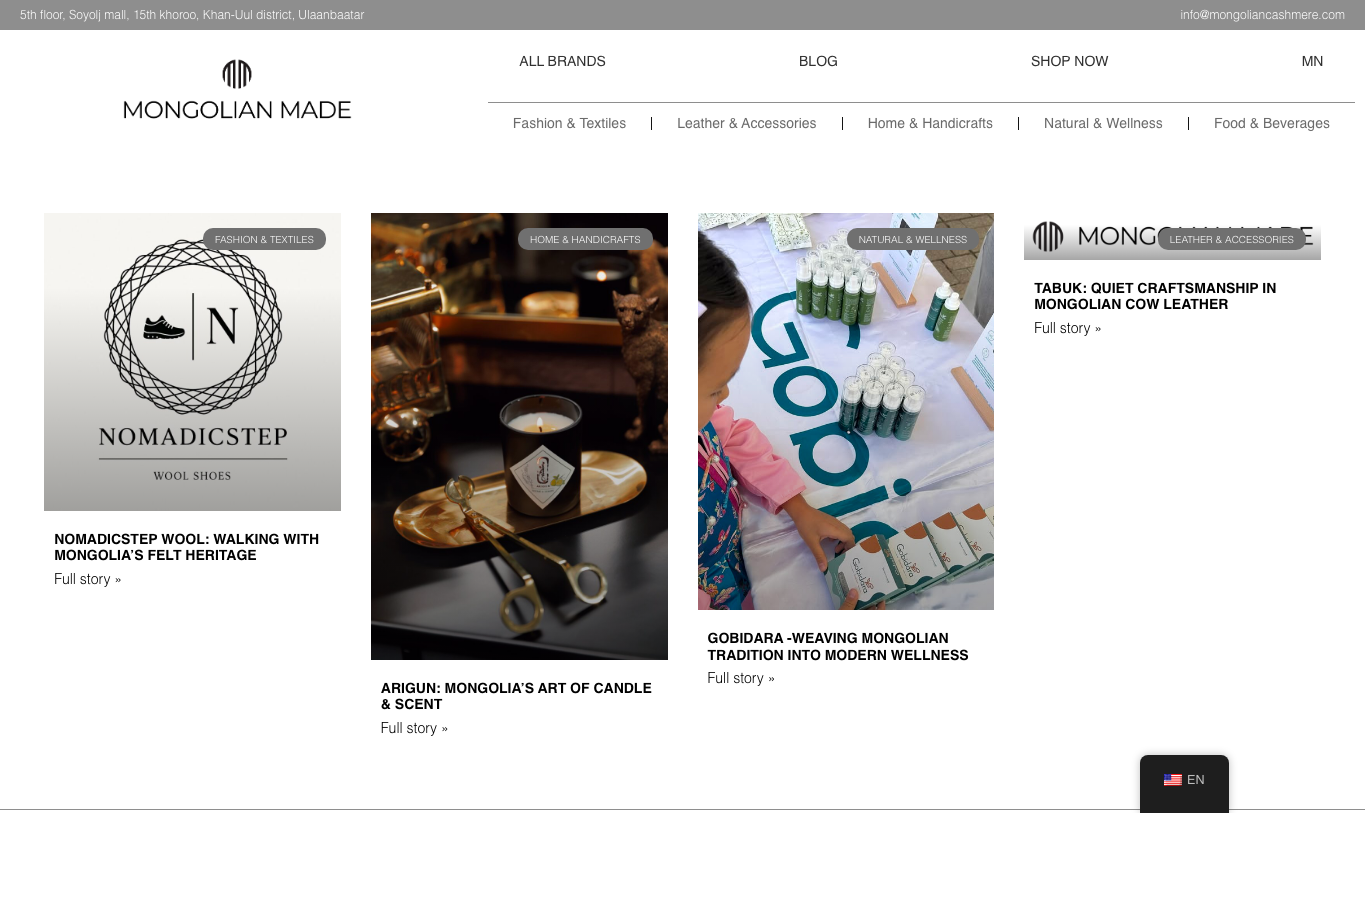
\includegraphics[width=0.45\textwidth]{Figures/similar_systems/mongolianmade.png}\hfill
  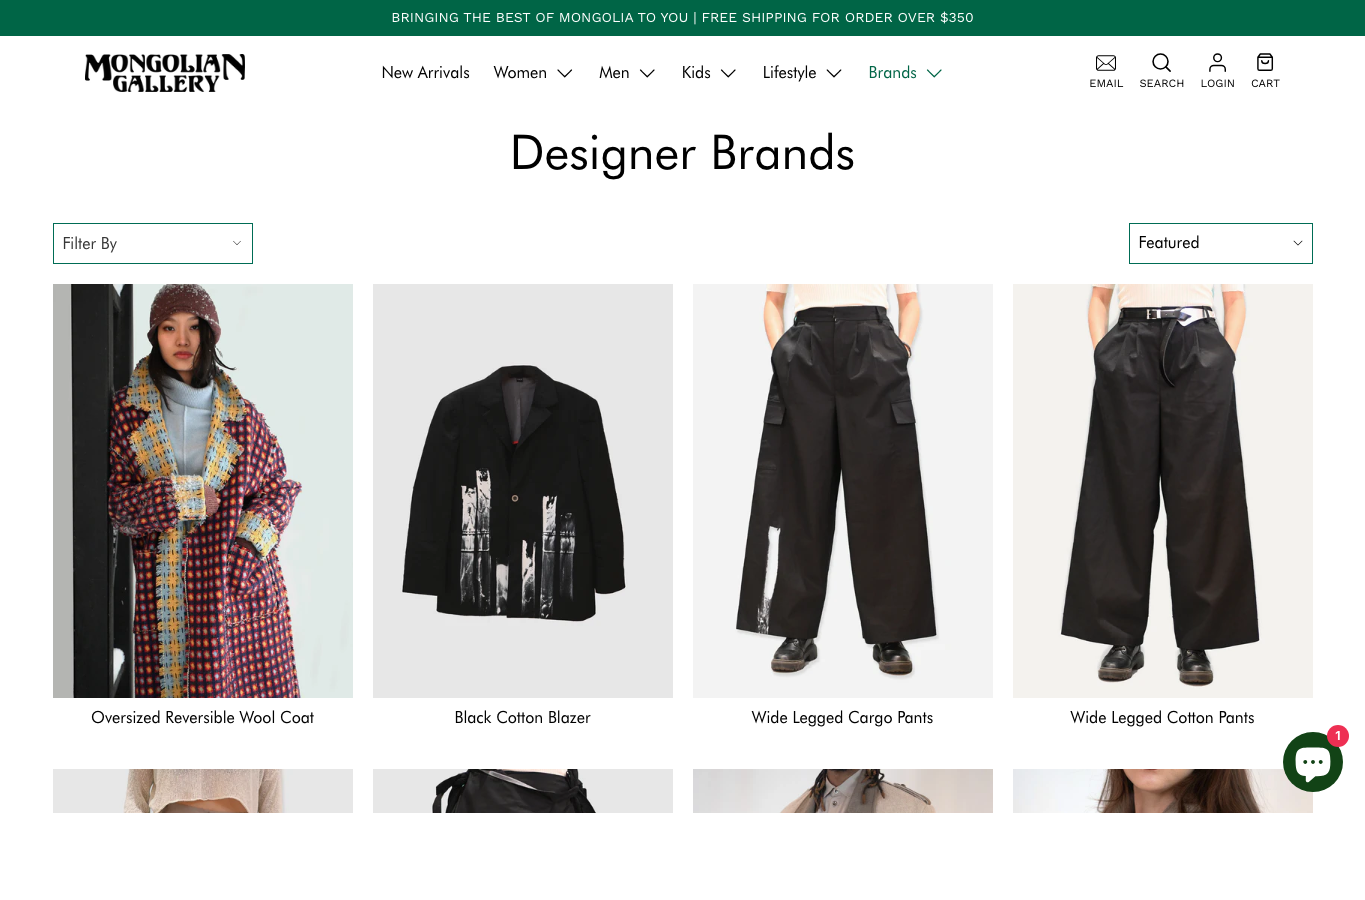
\includegraphics[width=0.45\textwidth]{Figures/similar_systems/mongolian_gallery.png}
  \caption[Монголын ижил төстэй вебүүдийн UI жишээ]{Монголын ижил төстэй вебүүдийн UI жишээ: Amulet, Deel, Gobi Cashmere, MongolianMade, Mongolian Gallery}
  \label{fig:mongolian-similar-screens}
\end{figure}

\subsection{Олон улсын ижил төстэй системүүд}
Олон улсын түвшинд Anoce/MFA-д ойр санаа өгөх таван системийг сонгов. Vogue Runway нь season, designer, latest show, image archive гэсэн бүтэцтэй runway/editorial архивын хамгийн танигдсан жишээний нэг \cite{vogue_runway_site}. Tagwalk нь fashion search engine хэлбэрээр collection, season, designer, model, trend, report, dashboard зэрэг хайлт-шинжилгээний боломжийг нэгтгэдэг \cite{tagwalk_site}. The Met Costume Institute нь музейн collection metadata, exhibition history, object preservation logic-оор хүчтэй \cite{met_costume_institute_site}. Google Arts \& Culture-ийн fashion project нь олон музей, curator story, theme, zoomable artifact, educational content-ийг холбодог \cite{google_arts_fashion_site}. CFDA Runway360 нь designer collection launch, press, sales, AR/VR, live video, e-commerce extension зэрэг digital showcase боломжийг нэг платформд нэгтгэх санааг харуулдаг \cite{cfda_runway360_site}.

{\small
\begin{longtable}{|L{0.15\textwidth}|L{0.17\textwidth}|L{0.32\textwidth}|L{0.22\textwidth}|}
  \caption{Олон улсын ижил төстэй системүүдийн шинжилгээ}
  \label{tab:international-similar-systems}\\
  \hline
  \textbf{Систем} & \textbf{Төрөл} & \textbf{Ажиллах зарчим ба UI шинж} & \textbf{Anoce/MFA-д авах санаа} \\ \hline
  Vogue Runway & Runway archive & Designer, season, show, gallery, review article-ийг нэгтгэнэ. UI нь өндөр чанартай runway зураг, clear navigation, editorial headline дээр тулгуурладаг. & Designer-season-collection relation, gallery + review хослуулах. \\ \hline
  Tagwalk & Fashion search engine & Collection, season, designer, model, trend, report, dashboard-оор хайх боломжтой. UI нь хайлт, filter, trend insight, result grid дээр төвлөрдөг. & Global search, tag taxonomy, trend/material keyword-г системтэй болгох. \\ \hline
  The Met Costume Institute & Museum archive & Object metadata, exhibition history, preservation, acquisition information-ийг баримтжуулна. UI нь музейн тайлбар, object detail дээр төвлөрдөг. & Item бүрт эх сурвалж, metadata, тайлбар хэрэглэх. \\ \hline
  Google Arts \& Culture Fashion & Culture platform & Museum partner, theme, story, zoomable image, lesson, curator narrative-г нэгтгэнэ. UI нь story card, image exploration, topic navigation дээр тулгуурладаг. & Archive-г curated story болон theme байдлаар үзүүлэх. \\ \hline
  CFDA Runway360 & Digital collection showcase & Designer launch page, press kit, show/product image, live stream, commerce/social integration зэрэг collection launch хэрэгслийг нэгтгэдэг. & Designer-д зориулсан modular profile болон collection launch workflow төлөвлөх. \\ \hline
\end{longtable}
}

\begin{figure}[htbp]
  \centering
  \IfFileExists{Figures/similar_systems/vogue_runway.png}{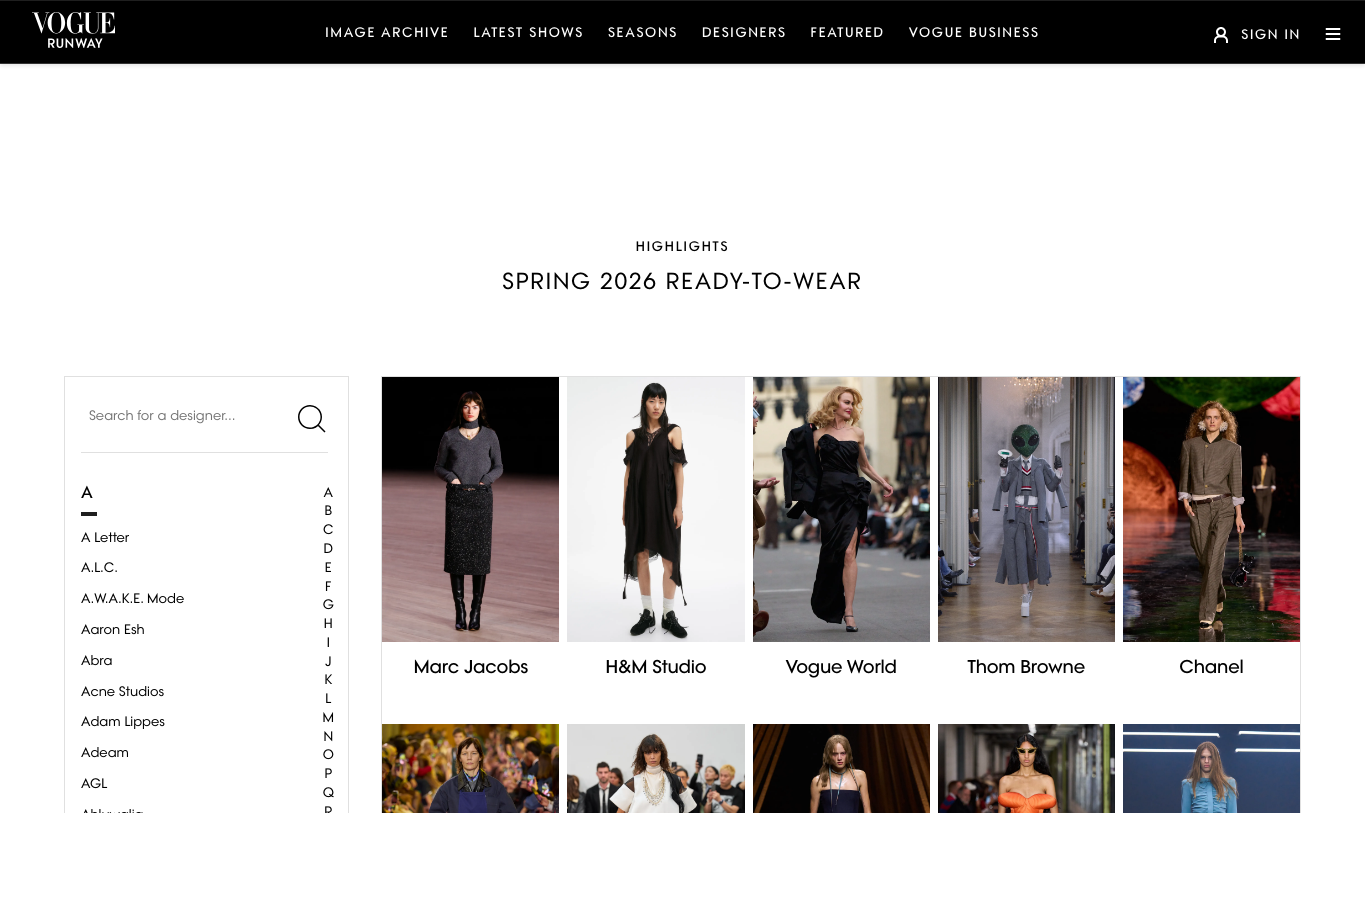
\includegraphics[width=0.31\textwidth]{Figures/similar_systems/vogue_runway.png}}{\fbox{\parbox[c][3.0cm][c]{0.31\textwidth}{\centering Vogue Runway\\official page}}}\hfill
  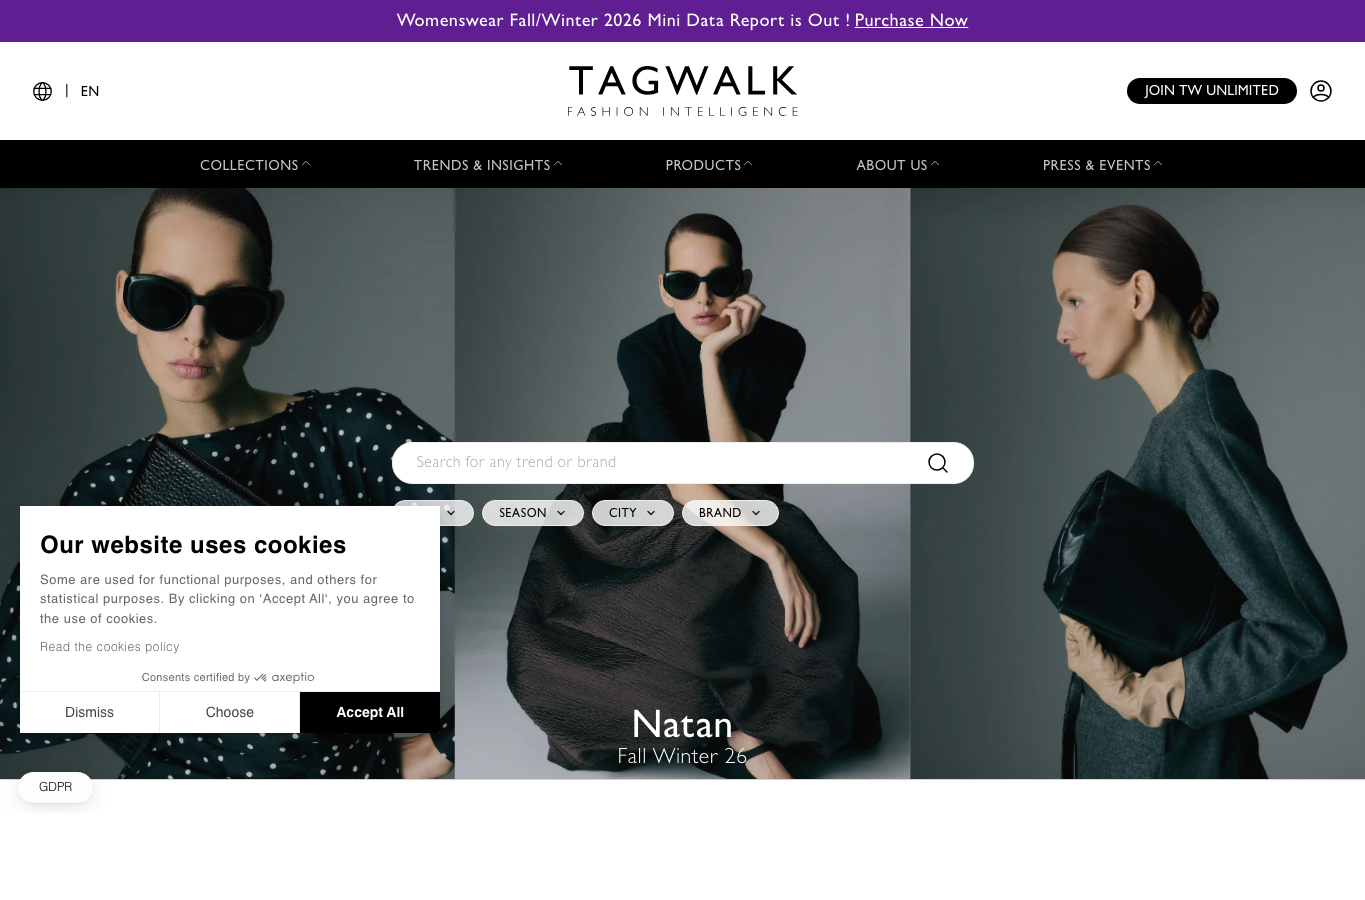
\includegraphics[width=0.31\textwidth]{Figures/similar_systems/tagwalk.png}\hfill
  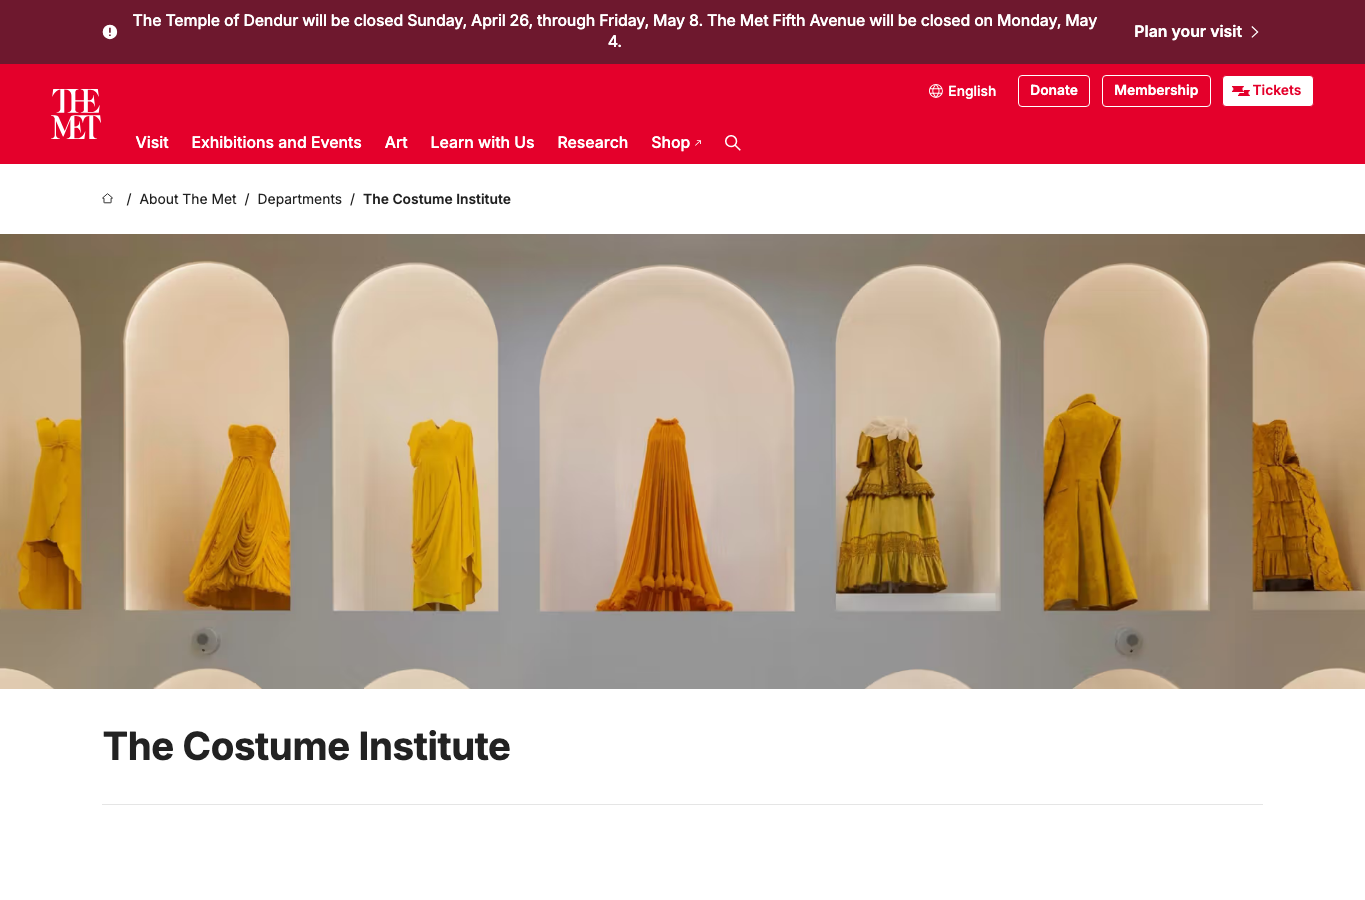
\includegraphics[width=0.31\textwidth]{Figures/similar_systems/met_costume.png}\\[0.6em]
  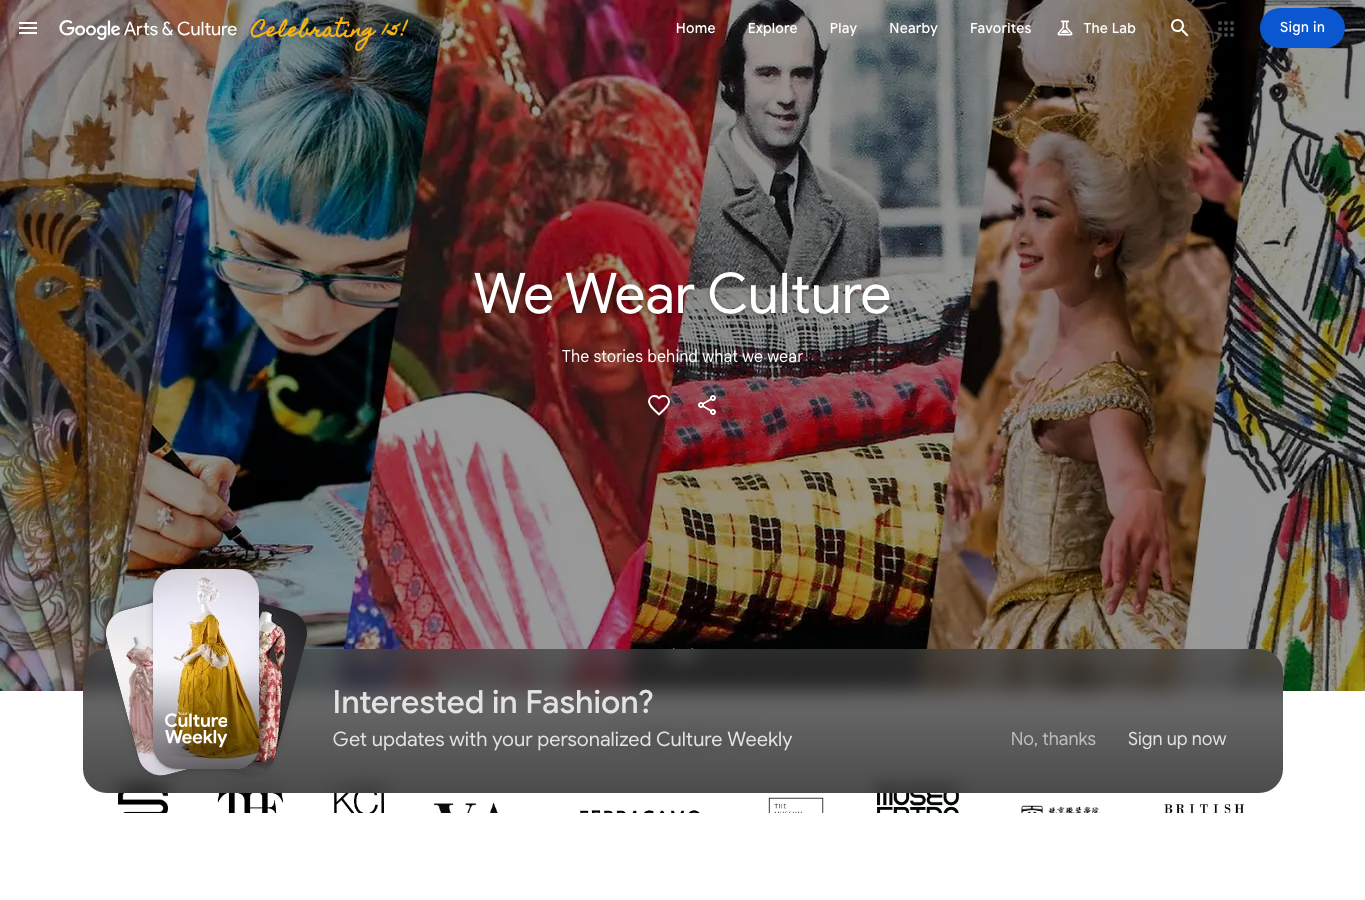
\includegraphics[width=0.45\textwidth]{Figures/similar_systems/google_fashion.png}\hfill
  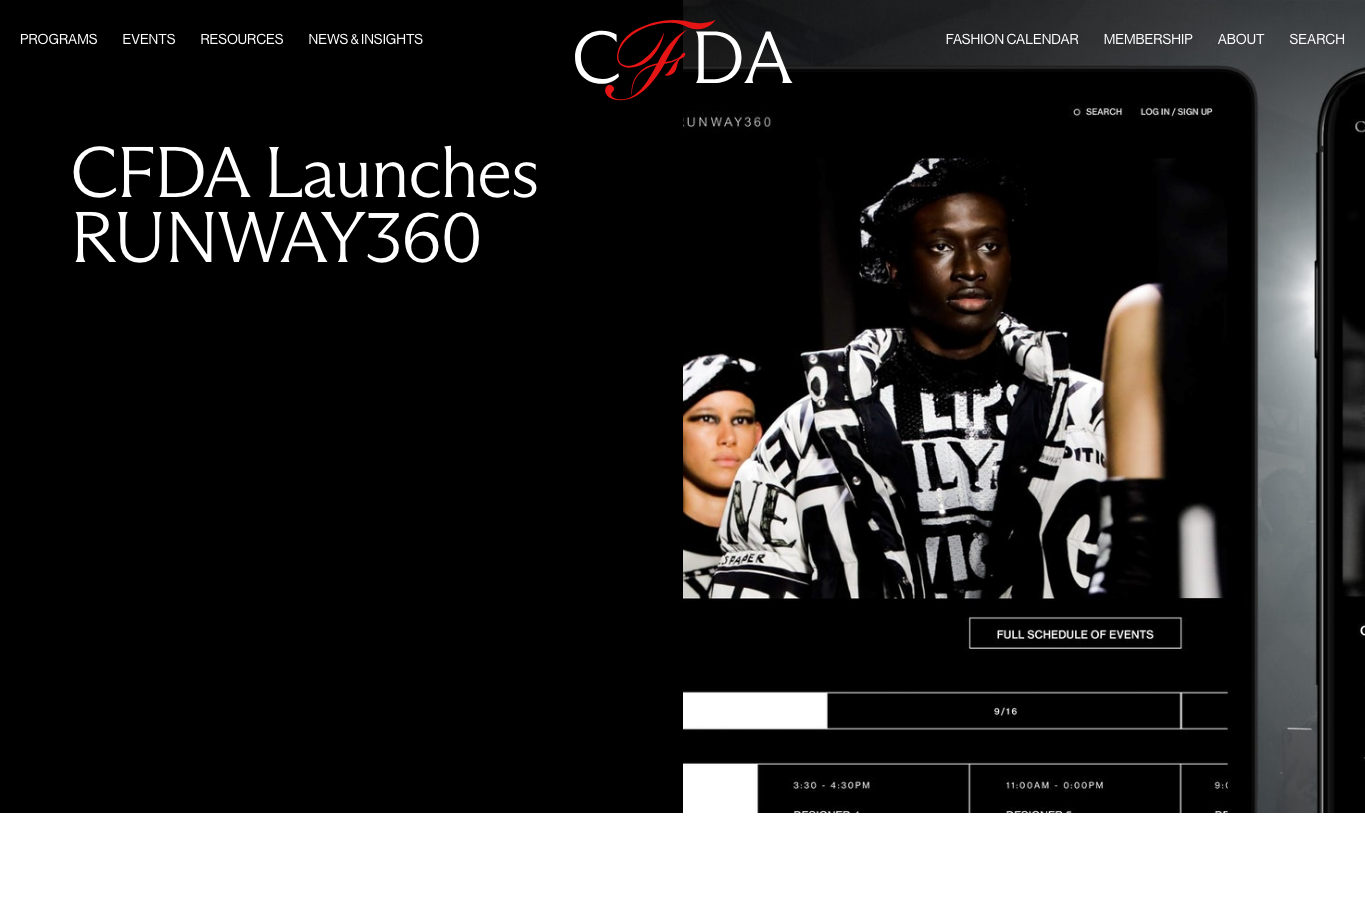
\includegraphics[width=0.45\textwidth]{Figures/similar_systems/cfda_runway360.png}
  \caption[Олон улсын ижил төстэй системүүдийн UI жишээ]{Олон улсын ижил төстэй системүүдийн UI жишээ: Vogue Runway, Tagwalk, The Met Costume Institute, Google Arts \& Culture Fashion, CFDA Runway360}
  \label{fig:international-similar-screens}
\end{figure}

\subsection{Судалгаанаас гарсан нэгтгэл}
Дээрх системүүдээс харахад Anoce/MFA платформд дараах зарчим чухал байна.
\begin{itemize}
  \item Зурагт суурилсан UI нь fashion archive-ийн анхны ойлголтыг хурдан өгдөг тул card, gallery, hero, detail layout-ийн чанар өндөр байх ёстой.
  \item Designer, collection, look, article, material, season, tag хоорондын relation тодорхой байхгүй бол хайлт болон AI туслах найдвартай ажиллахгүй.
  \item Монголын сайтууд brand/story талдаа хүчтэй боловч нэгдсэн archive metadata, cross-brand search, AI-assisted discovery харьцангуй сул байна.
  \item Олон улсын системүүд metadata, search, curated story, collection launch, museum credibility зэрэг тус тусын давуу талыг харуулж байна.
  \item Anoce/MFA нь эдгээр санааг нэгтгэн Монголын загварын салбарт тохирсон public archive, editorial CMS, global search, RAG chatbot бүхий платформ болгох боломжтой.
\end{itemize}

\section{Холбоотой судалгааны ажлууд}
Энэхүү төслийн арга зүйн үндэс нь программ хангамж хөгжүүлэх аргачлал, UX prototype, Design Science Research, AI/RAG системийн судалгаанаас бүрдэнэ. Waterfall нь дипломын баримтжуулалт, үе шат тодорхойлох тал дээр ашигтай боловч шаардлага өөрчлөгдөх веб бүтээгдэхүүнд дангаар тохиромжгүй \cite{royce_waterfall_1970}. Agile ба Kanban нь жижиг баг/ганцаарчилсан хөгжүүлэлтийн ажлыг давталттай, харагдахуйц удирдахад тохиромжтой \cite{agile_manifesto_2001,anderson_kanban_2010}. Design Science Research нь бодит артефакт бүтээж, судалгааны асуудалтай холбож үнэлэхэд тохиромжтой \cite{hevner_dsr_2004}.

\section{Систем хөгжүүлэх аргачлалуудын харьцуулалт}
Anoce/MFA платформын хөгжүүлэлтэд нэг аргачлал дангаараа хангалттай биш. Учир нь дипломын тайлан нь шинжилгээ, зохиомж, хэрэгжилт, үнэлгээ гэсэн дараалсан баримтжуулалт шаарддаг боловч бодит веб бүтээгдэхүүн нь UI prototype, content model, admin workflow, AI provider, RAG dataset зэрэг олон хэсэг дээр давталттай өөрчлөгддөг. Тиймээс аргачлалуудыг дараах шалгуураар харьцуулсан: шаардлага өөрчлөгдөхөд хариулах чадвар, UI/UX турших боломж, эрсдэлтэй хэсгийг хянах байдал, дипломын судалгааны contribution-ийг тайлбарлах чадвар, ганцаарчилсан хөгжүүлэлтийн ажлын зохион байгуулалт.

\subsection{Waterfall аргачлал}
Waterfall нь шаардлага, шинжилгээ, зохиомж, хэрэгжилт, туршилт, нэвтрүүлэлт гэсэн дараалсан бүтэцтэй \cite{royce_waterfall_1970}. Энэ аргачлал нь дипломын тайлангийн логикийг эмхлэхэд ашигтай: эхлээд асуудал, дараа нь технологи, хэрэгжилт, архитектур, туршилт гэсэн дараалал үүсгэнэ. Гэвч Anoce/MFA-ийн UI, content model, AI provider, admin workflow хөгжүүлэлтийн явцад олон удаа өөрчлөгдсөн. Иймээс Waterfall-ийг үндсэн хөгжүүлэлтийн арга бус, харин тайлангийн баримтжуулалт болон milestone шалгалтын хүрээ болгон ашиглах нь зохистой.

\subsection{Prototype аргачлал}
Prototype аргачлал нь visual archive, search overlay, admin table, article editor зэрэг хэрэглэгчийн интерфейсийг хурдан гаргаж, давталтаар сайжруулахад тохиромжтой. Fashion archive-ийн хувьд image ratio, card density, hero layout, filter ergonomics зэрэг шийдвэрийг зөвхөн текст шаардлагаар тодорхойлоход хангалтгүй. Тиймээс public homepage, archive card, search overlay, admin form зэрэг хэсгийг эхлээд ажиллах prototype байдлаар гаргаж, дараа нь өгөгдлийн model болон API-тай холбосон.

\subsection{Spiral аргачлал}
Spiral нь эрсдэлд суурилсан давталттай хөгжүүлэлт юм \cite{boehm_spiral_1988}. Энэ төсөлд AI chatbot, RAG dataset, provider fallback, admin authorization, asset upload зэрэг хэсэг эрсдэл өндөртэй. Жишээлбэл AI provider key байхгүй үед chatbot бүрэн ажиллахгүй болох, RAG dataset live content-оос хоцрох, viewer хэрэглэгч admin API дуудах зэрэг эрсдэл гарч болно. Spiral хандлагаар эдгээрийг жижиг туршилт болгон салгаж, fallback, role gate, context boundary, seed script зэрэг хамгаалалтыг давталтаар нэмсэн.

\subsection{Agile ба Kanban}
Agile нь ажиллаж буй бүтээгдэхүүнийг үе шаттай хүргэх, өөрчлөлтөд хурдан хариулах зарчимтай \cite{agile_manifesto_2001}. Kanban нь backlog, in progress, review, done гэсэн урсгалаар frontend, API, data, thesis бичвэрийг зэрэг хянахад тохиромжтой \cite{anderson_kanban_2010}. Бага баг эсвэл ганцаарчилсан дипломын хөгжүүлэлтэд Scrum-ийн formal ceremony бүрийг ашиглах шаардлагагүй ч Kanban board маягийн task visibility, small batch delivery, continuous review нь тохиромжтой.

\subsection{Design Science Research}
Design Science Research нь мэдээллийн системийн судалгаанд шинэ артефакт бүтээж, түүний хэрэгцээ, зохиомж, үнэлгээ, contribution-ийг тайлбарлах хандлага юм \cite{hevner_dsr_2004}. Энэ дипломын ажил нь бодит веб платформ, repository, admin CMS, AI chatbot, seed pipeline, LaTeX тайлан гэсэн артефактуудтай тул DSR хүрээтэй нийцнэ. DSR-ийн давуу тал нь кодын бүтээгдэхүүнийг судалгааны асуудалтай шууд холбож, ``ямар асуудал шийдэв, ямар артефакт бүтээв, яаж үнэлэв'' гэсэн логик үүсгэдэгт оршино.

\subsection{Lean UX ба хэрэглэгч төвтэй хандлага}
Lean UX нь урт хугацааны том specification бичихээс илүү hypothesis, prototype, feedback, learning loop ашиглан хэрэглэгчийн туршлагыг сайжруулах хандлага юм \cite{lean_ux_2013}. Anoce/MFA-д энэ нь archive browsing, filter visibility, search overlay, card density, admin form clarity зэрэг хэрэглэгч шууд мэдрэх хэсэгт ашигтай. Хэдийгээр албан ёсны хэрэглэгчийн том судалгаа хийгдээгүй ч UI heuristic review, responsive inspection, route scenario шалгалт нь Lean UX-ийн жижиг feedback loop хэлбэрээр ашиглагдсан.

\begin{longtable}{|L{0.15\textwidth}|L{0.22\textwidth}|L{0.22\textwidth}|L{0.27\textwidth}|}
  \caption{Аргачлалуудын харьцуулсан шинжилгээ}
  \label{tab:methodology-comparison}\\
  \hline
  \textbf{Аргачлал} & \textbf{Давуу тал} & \textbf{Сул тал} & \textbf{Энэ төсөлд тохирох байдал} \\ \hline
  Waterfall & Баримтжуулалт сайн, үе шат тодорхой & Өөрчлөлтөд уян хатан бус & Тайлан, шаардлага, диаграмыг цэгцлэхэд ашиглана. \\ \hline
  Prototype & UI/UX хурдан шалгана & Prototype code debt үүсгэж болно & Visual archive, search overlay, admin form-д тохиромжтой. \\ \hline
  Spiral & Эрсдэлийг давталтаар бууруулна & Процесс төвөгтэй байж болно & AI, RAG, auth, asset upload-д ашиглана. \\ \hline
  Agile ба Kanban & Давталттай хүргэлт, ажлын ил тод байдал & Ceremony-г багасгаж хэрэглэх шаардлагатай & Гол хөгжүүлэлтийн өдөр тутмын аргачлал. \\ \hline
  Lean UX & UI hypothesis-ийг хурдан шалгана & Том хэрэглэгчийн судалгааг бүрэн орлохгүй & Search, filter, card layout, admin form clarity-д ашиглана. \\ \hline
  Design Science Research & Судалгаа ба бүтээгдэхүүн холбогдоно & Үнэлгээний шалгуур тодорхой байх хэрэгтэй & Дипломын ерөнхий судалгааны хүрээ. \\ \hline
\end{longtable}

\section{Сонгосон арга зүйн загвар}
Дээрх харьцуулалтаас үзэхэд \textbf{DSR-д суурилсан Agile/Kanban хөгжүүлэлт, Prototype, Lean UX болон Spiral эрсдэлийн хяналтаар баяжуулсан} загварыг сонгов. Энэ загвар нь ажиллаж буй системийг хурдан хөгжүүлэх, интерфейсийг давталтаар сайжруулах, AI ба өгөгдлийн эрсдэлийг тусад нь шалгах, дипломын баримтжуулалтыг судалгааны логиктой хадгалах давуу талтай.

Сонгосон арга зүйн үндсэн логик нь дараах байдалтай. Нэгдүгээрт, DSR нь судалгааны асуудал, артефакт, үнэлгээний хүрээг тогтооно. Хоёрдугаарт, Agile/Kanban нь route, API, CMS, search, chatbot зэрэг ажлыг жижиг багц болгон явуулна. Гуравдугаарт, Prototype болон Lean UX нь public болон admin UI-ийн ойлгомжтой байдлыг давталтаар сайжруулна. Дөрөвдүгээрт, Spiral risk review нь AI, RAG, auth, asset, deployment зэрэг алдаа гарахад өндөр нөлөөтэй хэсгийг тусад нь шалгана.

\begin{table}[htbp]
  \centering
  \caption{Сонгосон арга зүйн бүрэлдэхүүн}
  \label{tab:selected-methodology}
  \begin{tabular}{|L{0.22\textwidth}|L{0.34\textwidth}|L{0.30\textwidth}|}
    \hline
    \textbf{Арга зүйн бүрэлдэхүүн} & \textbf{Төслийн хэрэглээ} & \textbf{Хүлээгдэж буй үр дүн} \\ \hline
    DSR & Судалгааны асуудал, артефакт, үнэлгээ тодорхойлох & Дипломын судалгаа ба кодын уялдаа баталгаажна. \\ \hline
    Agile/Kanban & Route, API, admin, chatbot, thesis ажлыг backlog-оор удирдах & Хөгжүүлэлт тасралтгүй, харагдахуйц болно. \\ \hline
    Prototype & Visual layout, search, admin form турших & UX шийдвэрийг хурдан шалгана. \\ \hline
    Lean UX & Card density, filter, responsive UI, admin form clarity-г давталтаар сайжруулах & Хэрэглэгчийн урсгал илүү ойлгомжтой болно. \\ \hline
    Spiral risk review & AI, RAG, auth, repository, asset upload эрсдэл шалгах & Эрсдэлтэй хэсэг бүрийн fallback ба boundary тодорхой болно. \\ \hline
  \end{tabular}
\end{table}

\section{Арга зүйн үе шат ба ажлын төлөвлөгөө}
\begin{enumerate}
  \item Судалгааны асуудал, хэрэглэгчийн хэрэгцээг тодорхойлох.
  \item Designer, collection, article, asset, user, RAG document entity-г загварчлах.
  \item Public archive, editorial, designer directory, search overlay-ийн prototype боловсруулах.
  \item CouchDB repository, content API, admin CMS, Supabase auth/role/bookmark холболт хэрэгжүүлэх.
  \item AI chatbot-ийн live archive search, Supabase RAG search, provider fallback-ийг турших.
  \item Use case, class, ER, sequence, deployment диаграм болон тайлангийн бүлгүүдийг боловсруулах.
  \item Route, API, lint, old-domain термин шалгалт хийж, дүгнэлт гаргах.
\end{enumerate}

\section{Үнэлгээний арга}
\begin{table}[htbp]
  \centering
  \caption{Үнэлгээний шалгуур}
  \label{tab:evaluation-criteria}
  \begin{tabular}{|p{0.20\textwidth}|p{0.36\textwidth}|p{0.32\textwidth}|}
    \hline
    \textbf{Шалгуур} & \textbf{Үнэлэх зүйл} & \textbf{Баримтлах арга} \\ \hline
    Функциональ бүрэн байдал & Public archive, admin CMS, search, chatbot ажиллах эсэх & Route scenario, manual UI check \\ \hline
    Өгөгдлийн загвар & Designer, collection, look, article, asset relation & Type, repository, seed script review \\ \hline
    Security & Admin role gate, API authorization, user bookmark ownership & Protected route/API scenario \\ \hline
    AI чанар & Хариулт live archive/RAG context-д тулгуурлаж байгаа эсэх & Sample prompt, fallback inspection \\ \hline
    UX ойлгомжтой байдал & Archive хайх, article унших, designer үзэх, admin засах урсгал & Heuristic review, responsive inspection \\ \hline
  \end{tabular}
\end{table}

\section{Бүлгийн дүгнэлт}
Нэгдүгээр бүлгээр Anoce/MFA веб платформын үндэслэл, хэрэглэгчийн хэрэгцээ, шаардлага, ижил төстэй системүүд болон хөгжүүлэх арга зүйг тодорхойлов. Судалгаанаас харахад энэ төсөл нь зөвхөн загварын landing page бус, харин content repository, CMS, global search, AI chatbot, user personalization-ийг нэгтгэсэн дижитал архивын систем юм. Иймээс DSR, Agile/Kanban, Prototype, Spiral risk review-ийн хосолсон арга зүйг сонгосон нь дараагийн технологи, хэрэгжилт, архитектурын бүлгүүдийн суурь болно.
